
\restartappendixnumbering
\renewcommand{\thefigure}{A\arabic{figure}}
\renewcommand{\theHfigure}{A\arabic{figure}}

% \section{\agu{Archetypal Systems}}
% \setcounter{figure}{0}
% \renewcommand{\figurename}{Figure A}
% \section{Archetypal Systems}
Below, we show modeling results for four types of typical systems: folds, cusps, crosses, and doubles. \begin{figure}[H]
    \centering
    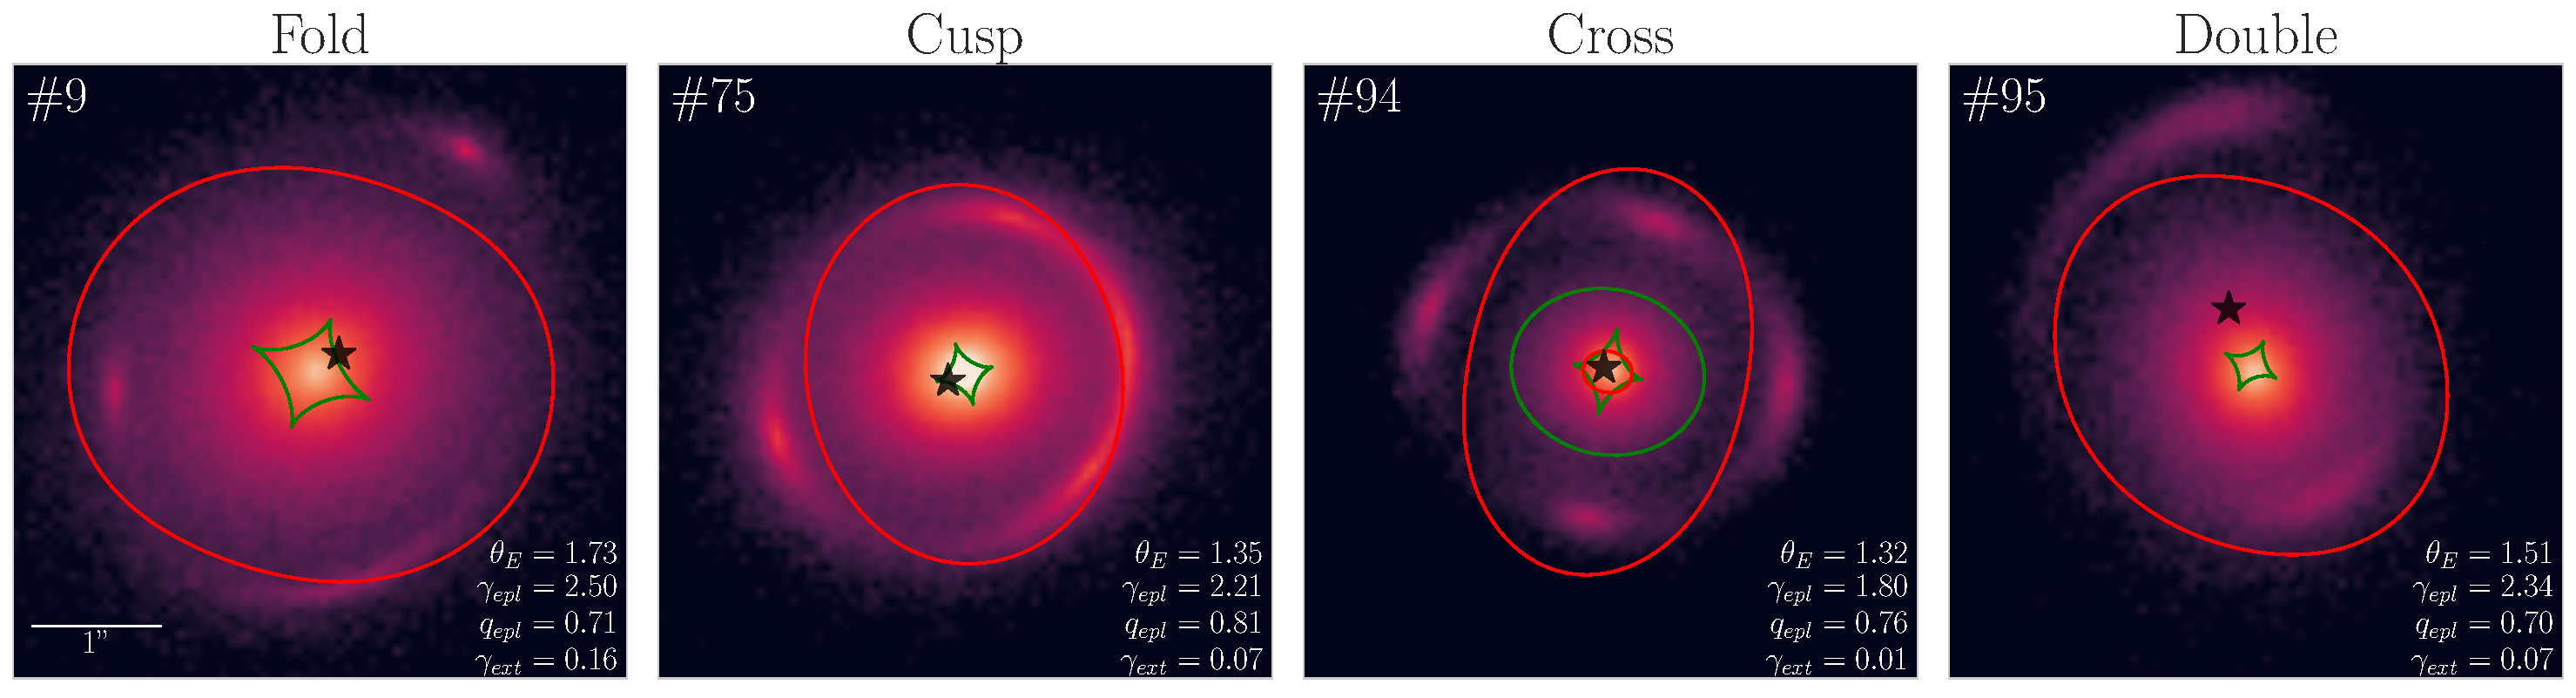
\includegraphics[width=0.9\textwidth]{figures/special-sys.pdf}
    \caption{Four archetypal lensing systems selected from \cref{fig:lens-sample}: a folds, cusps, crosses, and doubles. The numbers in the top left corner refer to the ordering in \cref{fig:lens-sample}. All four systems have a comparable SNR. The source location is marked with a star, the critical curves are in red, and the caustics are in green. Observe the presence of an inner critical curve and caustic in the cross system, due to the fact that $\gamma_{epl} < 2$ \citep[e.g.,][]{oriordan2019}.}
    \label{fig:special-sys}
\end{figure}
For all four systems, the posterior mean agrees (within uncertainty) with the ground truth. In the folds (a), we point out the clear banana-shaped posterior (for similar examples with cluster lensing, see \citet{jullo2007}), as well as the weaker constraint on $\gamma$ (the standard deviation is here $\pm 0.1$, compared to the more typical $\pm 0.05$ for the other systems). This is worth keeping in mind when doing density profile slope studies. Furthermore, note the tendency for the VI posterior in (a) to underestimate the posterior scale. In contrast, for the cusp (b), the VI posterior overestimates the posterior scale for $\theta_E$. Notably, for the cross system (c), the results are qualitatively similar to the results for the reference system (which is also an approximate cross). That is, the degree of agreement between the ground truth and posterior mean is comparable to that of the reference system, and in both cases, the marginals of the VI posterior are similar to those of the true posterior. Finally, for the double (d), the marginals of the VI nearly perfectly agree with those of the true posterior.
\begin{figure}[H] % gridlines dont work well with makebox
\gridline{\fig{figures/arch-0.pdf}{0.49\textwidth}{(a) Folds}
          \fig{figures/arch-1.pdf}{0.49\textwidth}{(b) Cusps}}
\gridline{\fig{figures/arch-2.pdf}{0.49\textwidth}{(c) Crosses}
          \fig{figures/arch-3.pdf}{0.49\textwidth}{(d) Doubles}}
\caption{Modeling results for each of the four archetypal systems. The samples and $0.5$, $1$, $1.5$, $2$ $\sigma$ contours (corresponding to roughly $12\%$, $39\%$, $68\%$, $86\%$ of the probability mass), for both VI and HMC are shown in blue and grey, respectively. \label{fig:archtypes}}
\end{figure}

% \section{Computational Graph}
% \restartappendixnumbering
% \renewcommand{\thefigure}{B\arabic{figure}}
% \renewcommand{\theHfigure}{B\arabic{figure}}


% In \cref{fig:comp-graph}, we show the computational graph for simulating one system using our framework, starting from the parameters (bottom), ending with one simulated image (top). The edges represent connections through which gradients flow. This is essentially a visual representation of how the chain rule is used for automatic differentiation.

% \begin{figure}[H]
%     \centering
%     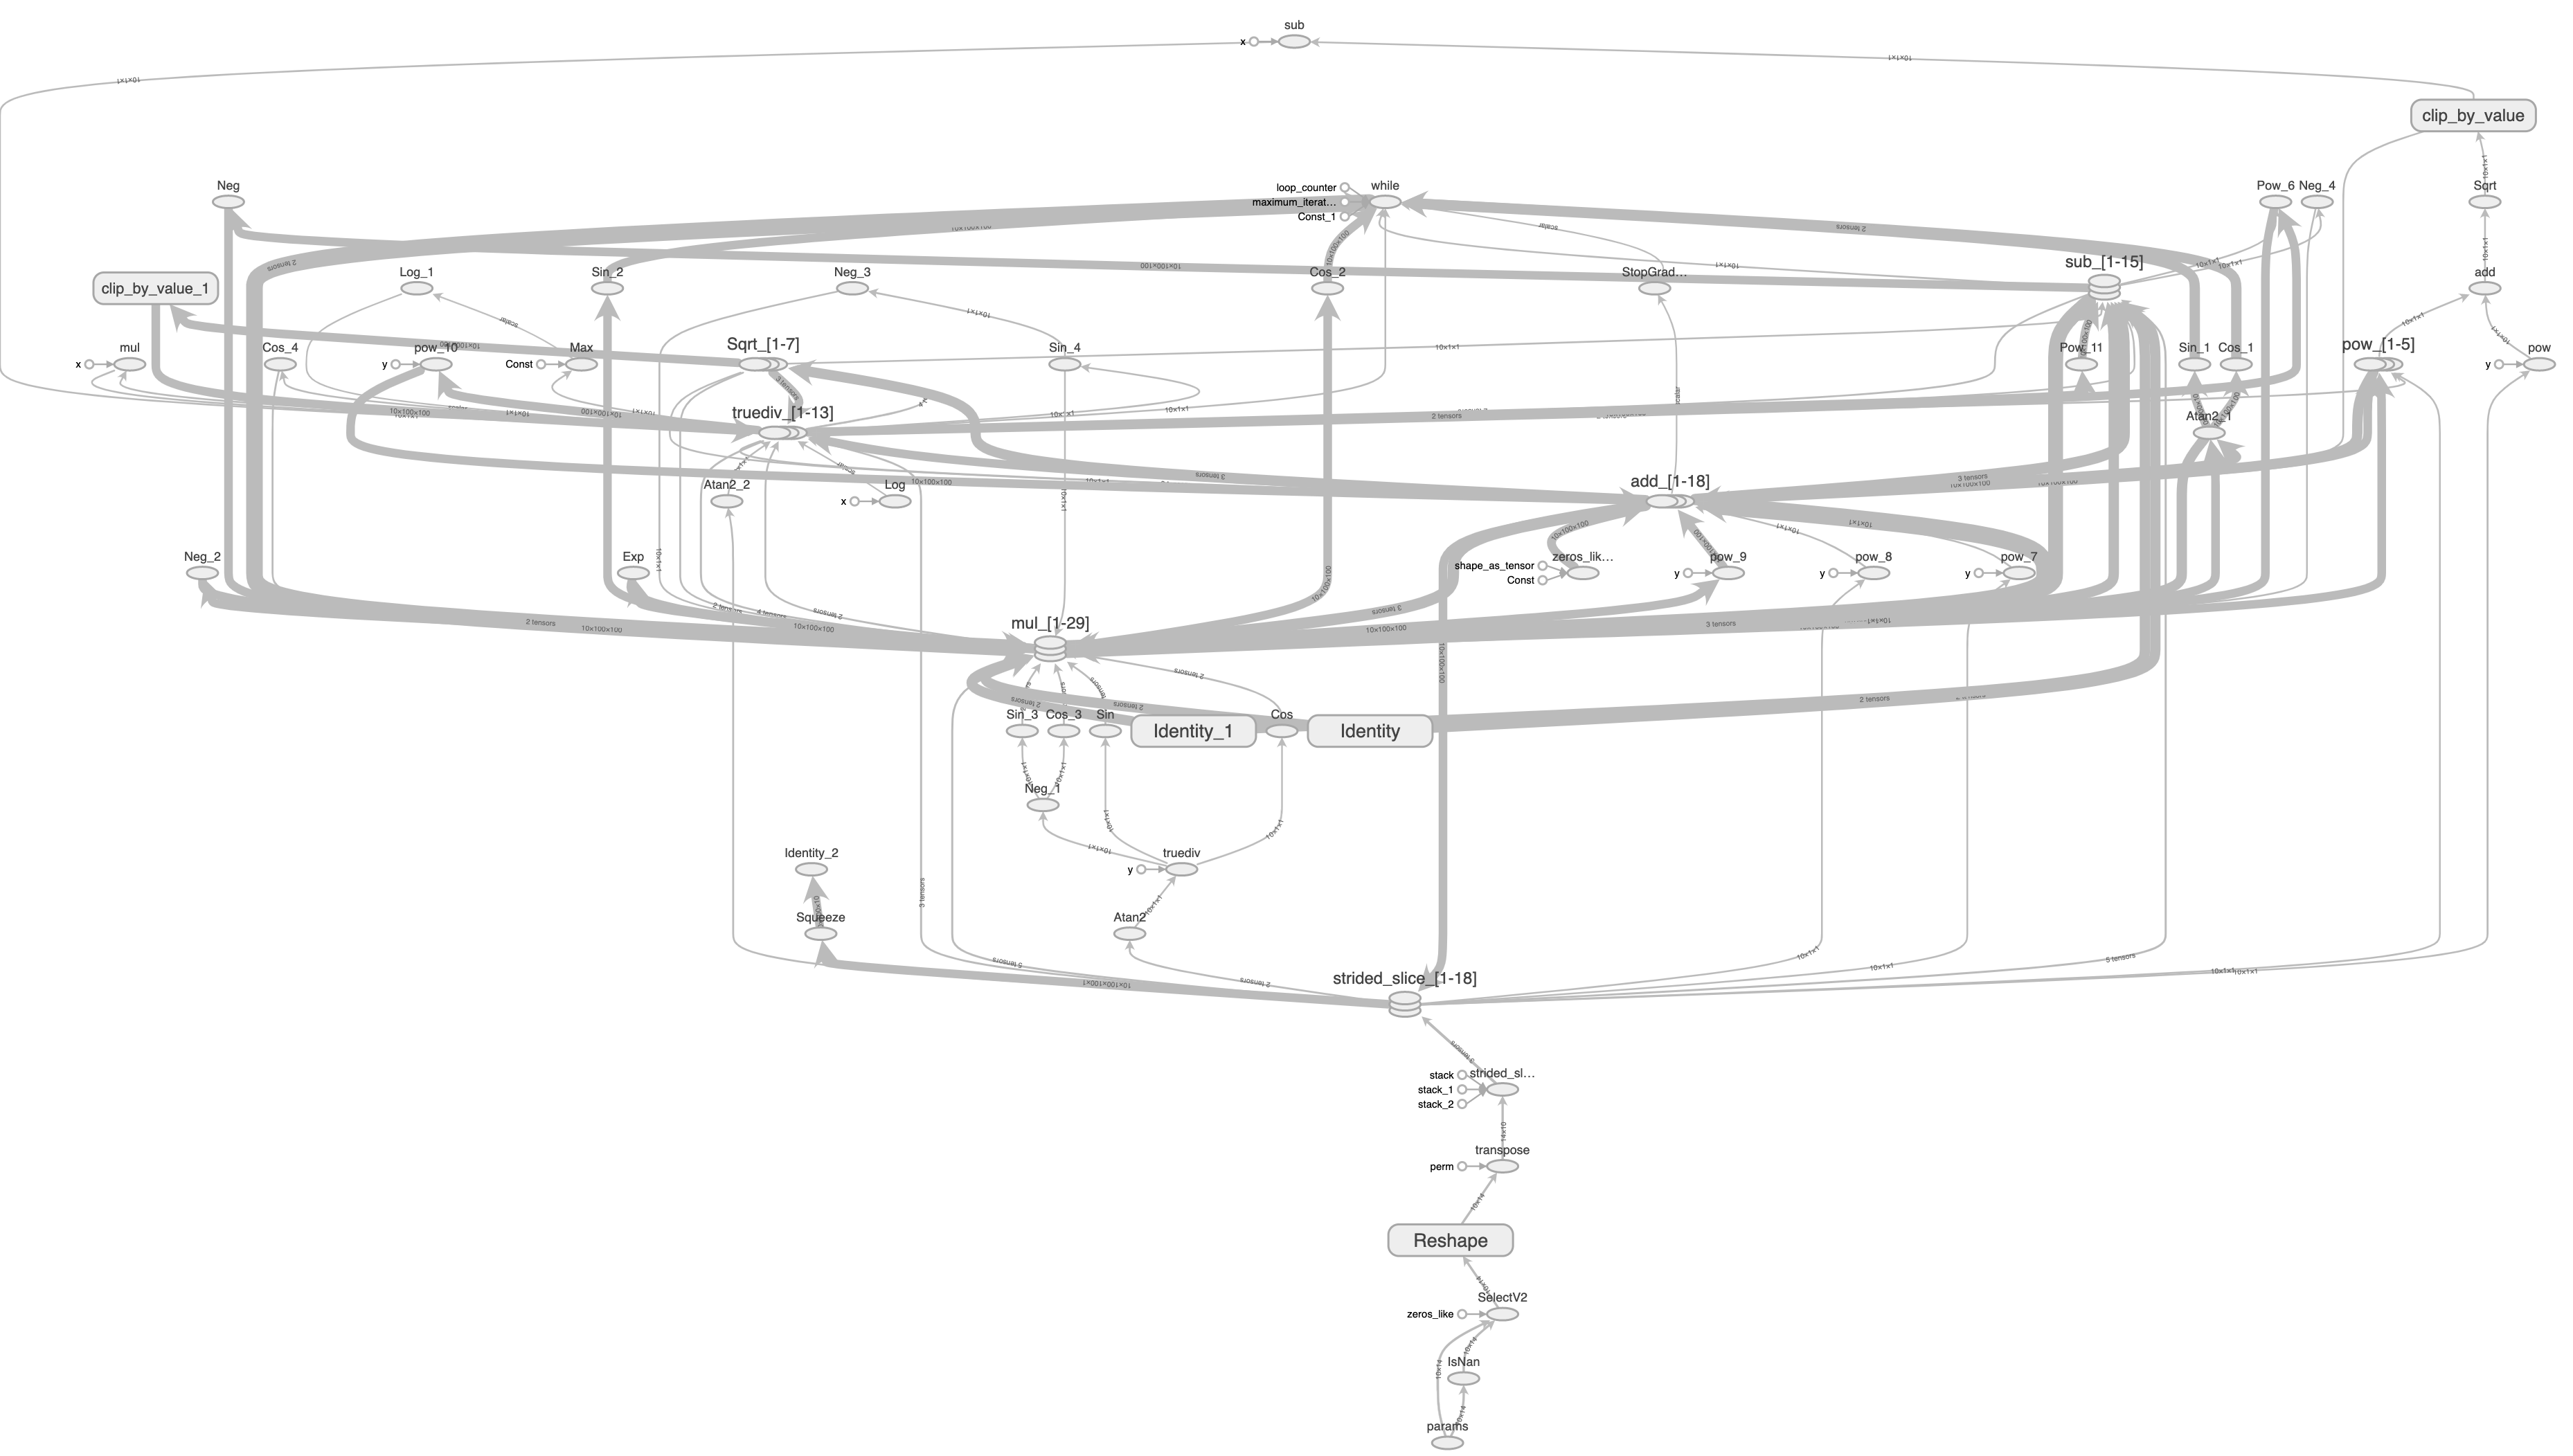
\includegraphics[width=\textwidth]{figures/comp-graph.png}
%     \caption{Computational graph for simulating one system. The nodes represent operations, while the edges represent pathways through which gradients flow.}
%     \label{fig:comp-graph}
% \end{figure}